
\section{Modernity}

CDCS is an old system, relatively speaking, and its development on user-facing features has been almost entirely stagnant. It launched in 2009, seven years ago, and has hardly changed since. Figure \ref{fig:cdcs2010} shows CDCS in July 2010, which, besides the addition of a few search fields, is identical to its current version. Yet, since its introduction in 2009, we have seen the rise of mobile devices into ubiquity, a boom in ``hacker culture'' and public APIs, and the capability for standalone web applications to be as sophisticated and dynamic as desktop-class applications without the aid of browser extensions. To this end, Skedge brings course scheduling to the modern era.

\begin{figure}[ht]
  \centering
    \fbox{
      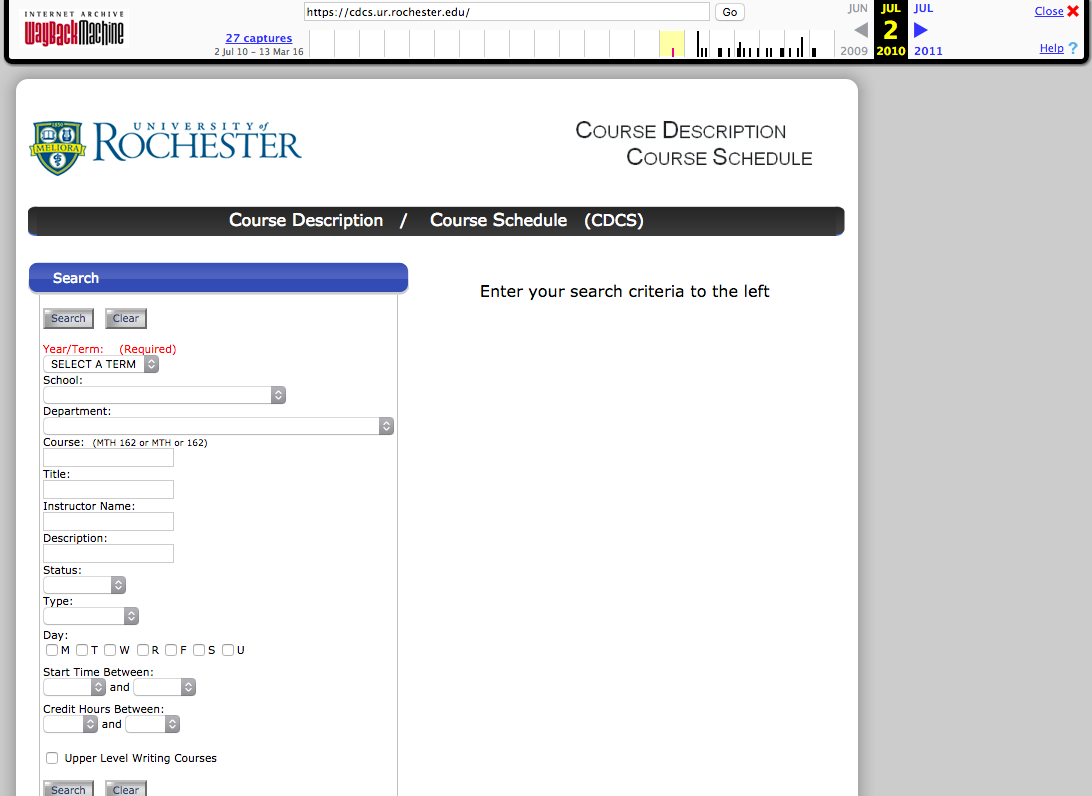
\includegraphics[width=10cm]{images/cdcs/2010}
    }
  \caption[CDCS in July 2, 2010]{CDCS in July 2, 2010, virtually unchanged from today, courtesy of \emph{Archive.org}\cite{archive}}
  \label{fig:cdcs2010}
\end{figure}

\subsection{AJAX vs. GET requests}

CDCS makes an AJAX request with every submitted search, meaning that the server receives the request and returns a response all without any page navigation (i.e. the URL stays the same and no new page is loaded as the search results are displayed). Skedge, however, makes a GET request for every search submission, meaning that the user's browser loads a new page that contains the results and whose URL reflects the search query. This simple technical design decision substantially increases usability for two reasons:

\begin{enumerate}
  \item Page navigations allow users to leverage their browser history as it was designed---after making several searches, CDCS users who use the back button on their browsers will be brought to the page loaded before the very first use of CDCS, possibly losing time spent in crafting sophisticated searches. Skedge users can go backwards and forwards through their search histories and scroll locations using native browser functionality.
  \item Every search query has a unique URL (e.g. \url{http://skedgeur.com/?q=csc} for {\tt csc}), so users are able to send links to a specific course or search result to others. With CDCS, the URL remains \url{https://cdcs.ur.rochester.edu} throughout the duration of the session.
\end{enumerate}


\subsection{Mobile}

According to Mary Meeker's 2015 Mobile Technology Trends from Kleiner Perkins Caufield \& Byers\cite{kpcb}, in 2014, 51\% of adult time spent per day on the Internet was from a mobile device, versus 42\% spent on a desktop computer or laptop. Time spent on the Internet with mobile devices reached three hours per day in 2014, compared to less than one hour in 2010 (when there was 12\% mobile vs. 75\% desktop/laptop time share).

Undeniably, supporting mobile devices and tablets in web applications is crucial for usability nowadays. Note how Skedge responds to the device form-factor in Figure \ref{fig:sk-mobile}, compared with CDCS's lack of mobile support in Figure \ref{fig:cdcs-mobile}. CDCS on mobile requires the user to pinch and drag around both to read results and to make new searchs, while Skedge adapts content to the device's screen and fixes the search bar to the top of the screen for easy access while browsing.

Moreover, since no major mobile browser currently supports browser extensions (and if one did, the extensions themselves would most likely need to be re-architected), CDCS on a mobile device loses all scheduling functionality, unlike Skedge, which supports it.

\begin{figure}[ht]
  \centering
  \vspace{10pt}
  \begin{tabular}{c c}
    \begin{subfigure}[h]{4.8cm}
      \centering
      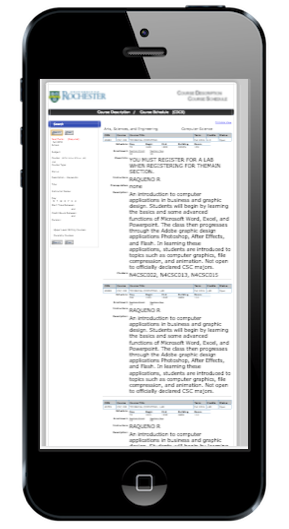
\includegraphics[width=1.00\textwidth]{images/cdcs/mobile}
      \caption{CDCS} \label{fig:cdcs-mobile}
    \end{subfigure}
    \begin{subfigure}[h]{4.7cm}
      \centering
      
\includegraphics[width=1.00\textwidth]{images/skedge/mobile}
      \caption{Skedge} \label{fig:sk-mobile}
    \end{subfigure}
  \end{tabular}
  \caption{CDCS and Skedge on a mobile browser}
\end{figure}

\subsection{Public API}

With the increasing number of attendees at University of Rochester's hackathons, it is clear that the University's ``hacker culture'' is growing---more students are collaborating to build side-projects that integrate resources and services often benefitting the student community. Open-source and open-information services greatly help to foster such innovation, and having public APIs is essential toward this end \cite{Milberry} \cite{hackers}.

Skedge provides a public JSON API at the root URL \url{http://www.skedgeur.com/api/}, originally made at the request of a student that was interested in using course data, and the API has since been used in projects by several other student groups. The endpoints included as of now are \url{/api/courses?q=query} (Skedge's query language---described in detail in section 2.3---is supported here) and \url{/api/departments} for a list of department names and codes.

\subsection{Built-in scheduler}

Skedge offers users a course schedule right in the page, unlike CDCS which requires the Better CDCS browser extension. Having a native schedule has several advantages:

\begin{enumerate}
\item Besides some CDCS users possibly not even knowing about Better CDCS, not requiring a browser extension provides for a faster and more seamless user onboarding, especially when building schedules on public computers where extensions can't always be installed.

\item Skedge was designed with a native schedule in mind, whereas Better CDCS works within an interface that wasn't. CDCS suffers from lower usability as a result, requiring the user to toggle between results and the schedule. Skedge, conversely, provides immediate visual feedback on how courses fit∫ into the user's schedule when the cursor is hovered over them.

\item Schedule data is centralized on Skedge's servers as opposed to locally in a browser, meaning that it can synchronize across a user's devices and can be easily publicly shared to others.

\item Extensions like Better CDCS have limited browser support. Internet Explorer and mobile browsers are unsupported, for example.

\item As separate systems trying to deliver one cohesive experience, Better CDCS and CDCS are dependent on each other. If the format of one changes, the other is likely to break.
\end{enumerate}
